
% This LaTeX was auto-generated from MATLAB code.
% To make changes, update the MATLAB code and republish this document.

\documentclass{article}
\usepackage{graphicx}
\usepackage{color}

\sloppy
\definecolor{lightgray}{gray}{0.5}
\setlength{\parindent}{0pt}

\begin{document}

    
    
\section*{Q1 - Root Locus Design}


\subsection*{Contents}

\begin{itemize}
\setlength{\itemsep}{-1ex}
   \item Get the Plant
   \item Need poles with real \ensuremath{>}= 15.3 or \ensuremath{<}= 6.7 (to satisy 2 away from plant poles)
   \item Set up PI controller
\end{itemize}


\subsection*{Get the Plant}

\begin{verbatim}
clc; clear all;

% figure(1); clf;

% need to find range of pid zeros (cant be less than 2 away from real of poles)
%G = ece414planttf(6,10,.45)
% figure(1); clf;
% for i = 0:1:9
%     G = ece414planttf(6,10,i/10);
%     rlocus(G))
%     grid on
%     axis([-20 0 -25 25]);
%     hold on
% end
% legend(['alpha = ' num2str(0)],['alpha = ' num2str(.1)],['alpha = ' num2str(0.2)],['alpha = ' num2str(0.3)], ['alpha = ' num2str(0.4)], ['alpha = ' num2str(0.5)], ['alpha = ' num2str(0.6)], ['alpha = ' num2str(0.7)], ['alpha = ' num2str(0.8)], ['alpha = ' num2str(0.9)]);
\end{verbatim}


\subsection*{Need poles with real \ensuremath{>}= 15.3 or \ensuremath{<}= 6.7 (to satisy 2 away from plant poles)}

\begin{par}
only adding pole at origin so were ok
\end{par} \vspace{1em}
\begin{verbatim}
% -12.8, -13.3, -11.4, -12, -9.12, -8.66
% rlocus(G)
% xlim([-20 5])
% ylim([-30 30])
 s=tf('s');
% %unity gain feedback
% % figure(3); clf;
% % Need at least I, as we need pole at origin for ess=0, kd makes it
% % improper so will not use
%

% G = ece414planttf(6,10,.45)
\end{verbatim}


\subsection*{Set up PI controller}

\begin{verbatim}
z = 15;
k = 30;
D = (k * (s + z))/s
% figure(2); clf;
% rlocus(D)


% figure(4); clf;
% rlocus(L)
disp('Alpha = .5')
G = ece414planttf(6,10,.5);
L = D*G;
T = feedback(L,1);
figure(1); clf;
step(T);
axis([0 2.5 0 1.1])
U = D/(1+L);
info = stepinfo(U);
peak = info.Peak
info = margins(L);
PM = info.Pm
info = stepinfo(T);
tr = info.RiseTime
OS = info.Overshoot
ts = info.SettlingTime
[Smax,Wsp]=PeakSens(L);
disp('Peak Sensitivity = ');
disp(Smax);

disp('Alpha = .99')
G = ece414planttf(6,10,.99);
L = D*G;
T = feedback(L,1);
figure(2); clf;
step(T);
axis([0 2.5 0 1.1])
U = D/(1+L);
info = stepinfo(U);
peak = info.Peak
info = margins(L);
PM = info.Pm
info = stepinfo(T);
tr = info.RiseTime
OS = info.Overshoot
ts = info.SettlingTime
[Smax,Wsp]=PeakSens(L);
disp('Peak Sensitivity = ');
disp(Smax);
\end{verbatim}

        \color{lightgray} \begin{verbatim}
D =
 
  30 s + 450
  ----------
      s
 
Continuous-time transfer function.

Alpha = .5

peak =

  104.8444


PM =

   65.9776


tr =

    0.2616


OS =

    0.8700


ts =

    0.4380

Peak Sensitivity = 
    1.4670

Alpha = .99

peak =

  226.3560


PM =

   83.2822


tr =

    0.9609


OS =

     0


ts =

    1.7856

Peak Sensitivity = 
    1.1237

\end{verbatim} \color{black}
    
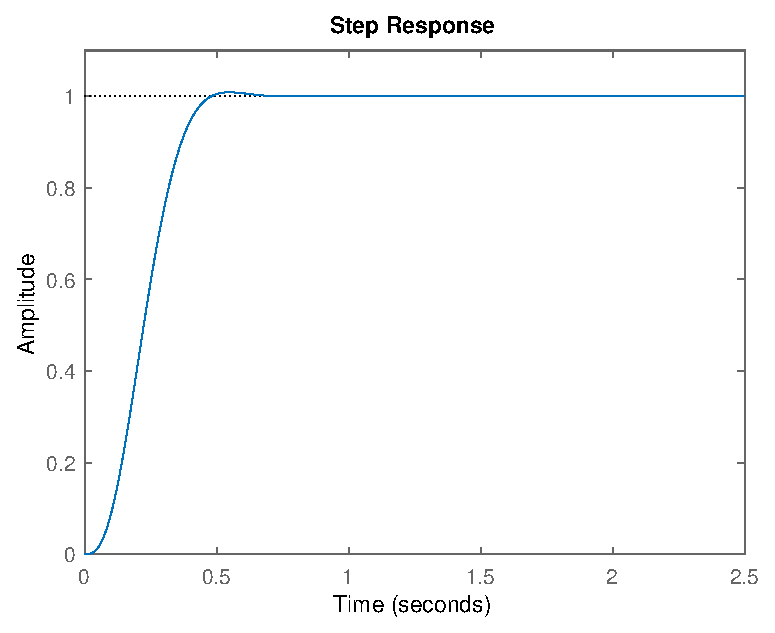
\includegraphics [width=4in]{Takehome_Q1_01.eps}

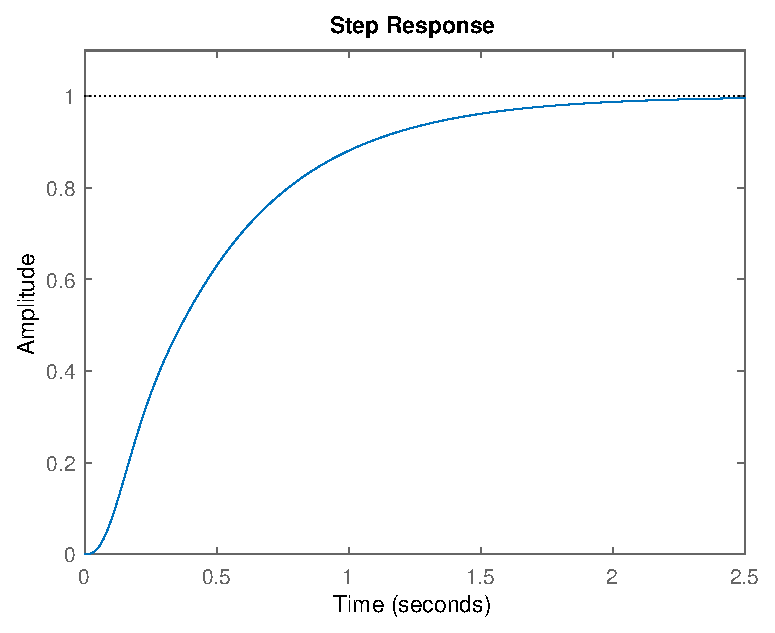
\includegraphics [width=4in]{Takehome_Q1_02.eps}



\end{document}
    
